\chapter{Basic Operations in Riemannian Space}
\pagebreak[4]

\section{p27-exercise}

\begin{tcolorbox}
Take polar coordinates $r, \theta$ in a plane. Draw the infinitesimal triangle with vertices $(r,\theta)$, $(r+dr,\theta)$, $(r,\theta + d\theta)$. Evaluate the square on the hypotenuse of this infinitisimal triangle, and so obtain the metric tensor for the plan for the coordinates$(r, \theta)$.\end{tcolorbox}
\begin{figure}[htp] 
    \centering
\includegraphics[scale=.5]{polar.jpg}
\end{figure}
\begin{align} 
\ ds^2 &= |AB|^2\\
\ &= dr^2 +|CA|^2\\
\ |CA| &= r\sin(d\theta)\approx rd\theta\\
\Rightarrow ds^2 &= dr^2 + r^2d\theta^2\\
\Rightarrow (a_{mn}) &= \begin{pmatrix}
 1& 0 \\
0 & r^2 \\
\end{pmatrix}
\end{align}
$$\medblackdiamond$$
\pagebreak[4]

\section{p27-exercise}

\begin{tcolorbox}
Show that if $x^1 = r, x^2 = \theta, x^3 = \phi$, in the usual notation of spherical polar coordinates, then $$ a_{11} =1, a_{22} = r^2, a_{33} = r^2\sin^2\theta$$ and the other components vanish.
\end{tcolorbox}
\begin{figure}[h]
\centering
\begin{minipage}[t]{.5\textwidth}
%\centering
\vspace{0pt}
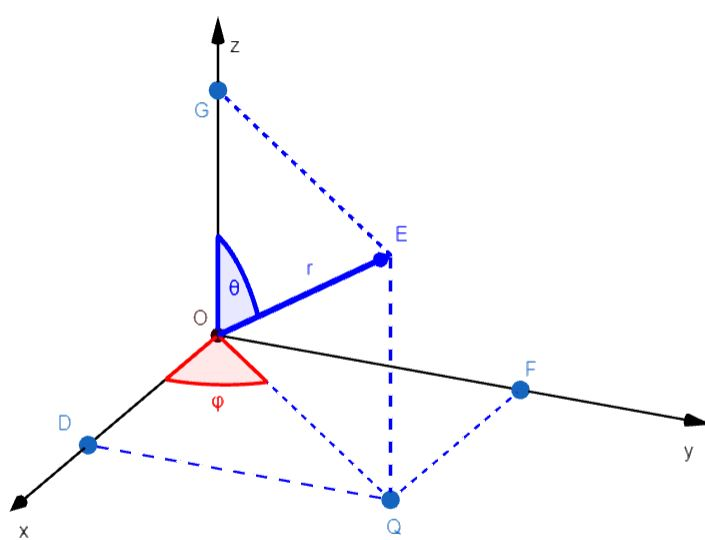
\includegraphics[scale=.5]{spherical.jpg}
\end{minipage}\hfill
\begin{minipage}[t]{0.4\textwidth}
%\centering
\vspace{50pt}
We use the latitude $\psi$ instead of the co-latitude $\phi$.\\\\
$\left\{ \begin{array}{c}
    x= r\cos (\psi )\cos (\theta) \\
     y= r\cos (\psi )\sin (\theta) \\
      z= r\sin(\psi )
  \end{array} \right.$
\end{minipage}
\end{figure}
\begin{align} 
\ ds^2 = dx^2 + dy^2 + dz^2\quad\text{with}\\
\left.
\begin{array}{c}
    dx= dr\cos (\psi )\cos (\theta)- r\sin (\psi )d\psi\cos (\theta) -r\cos (\psi )\sin (\theta)d\theta\\
     dy= dr\cos (\psi )\sin (\theta) -r\sin (\psi )d\psi\sin (\theta)+r\cos (\psi )\cos (\theta)d\theta\\
      dz= dr\sin(\psi )+r\cos(\psi )d\psi\\
  \end{array} \right\}
  \end{align}
  \begin{align}
  \left.
  \begin{array}{c}
    dx^2=
    \cos^2 (\psi )\cos^2 (\theta)dr^2\\- r^2\sin^2 (\psi )\cos^2 (\theta)d\psi^2\\ -r^2\cos^2 (\psi )\sin^2 (\theta)d\theta^2\\
    -\cos (\psi )\cos (\theta) r\sin (\psi )\cos (\theta)drd\psi\\
    -\cos (\psi )\cos (\theta)r\cos (\psi )\sin (\theta)drd\theta\\
    +r\sin (\psi )\cos (\theta)r\cos (\psi )\sin (\theta)d\psi d\theta  \\\\
     dy^2=  \cos^2 (\psi )\sin^2 (\theta)dr^2\\ +r^2\sin^2 (\psi )\sin^2 (\theta)d\psi^2\\+r^2\cos^2 (\psi )\cos^2 (\theta)d\theta^2\\-\cos (\psi )\sin (\theta)r\sin (\psi )\sin (\theta)dr d\psi\\ - \cos (\psi )\sin (\theta)r\cos (\psi )\cos (\theta)drd\theta\\
     -r\sin (\psi )\sin (\theta)r\cos (\psi )\cos (\theta)d\psi d\theta\\\\
      dz^2= \sin^2(\psi )dr^2 +r^2\cos^2(\psi )d\psi^2 + r\sin(\psi )\cos(\psi )drd\psi\\
  \end{array} \right\}
\end{align}
Rearrange terms:
  \begin{align}
  \left.
  \begin{array}{c}
    dx^2=
    \cos^2 (\psi )\cos^2 (\theta)dr^2\\+ r^2\sin^2 (\psi )\cos^2 (\theta)d\psi^2\\ +r^2\cos^2 (\psi )\sin^2 (\theta)d\theta^2\\
    -r\cos (\psi )\sin (\psi )\cos^2 (\theta)drd\psi\\
    -r\cos^2 (\psi )\cos (\theta)\sin (\theta)drd\theta\\
    +r^2\sin (\psi )\cos (\theta) \cos (\psi )\sin (\theta)d\psi d\theta  \\\\
     dy^2=  \cos^2 (\psi )\sin^2 (\theta)dr^2\\ +r^2\sin^2 (\psi )\sin^2 (\theta)d\psi^2\\+r^2\cos^2 (\psi )\cos^2 (\theta)d\theta^2\\-r\cos (\psi )\sin (\psi )\sin^2 (\theta)dr d\psi\\ - r\cos^2 (\psi )\sin (\theta) \cos (\theta)drd\theta\\
     -r^2\sin (\psi )\sin (\theta)\cos (\psi )\cos (\theta)d\psi d\theta\\\\
      dz^2= \sin^2(\psi )dr^2 +r^2\cos^2(\psi )d\psi^2 + r\sin(\psi )\cos(\psi )drd\psi\\
  \end{array} 
  \right\}
\end{align}
Grouping similar infinitesimal components and using basic trigonometric identities gives:
\begin{align}
\ ds^2 &= dr^2 +  r^2d\psi^2 + r^2\cos^2(\psi)d\theta^2\\
\text{replace  }\psi\text{ with } \frac{\pi}{2}-\phi \Rightarrow ds^2 &= dr^2 +  r^2d\phi^2 + r^2\sin^2(\phi)d\theta^2\\
\Rightarrow (a_{mn}) &= \begin{pmatrix}
 1& 0 & 0\\
0 & r^2 & 0 \\
0 & 0 & r^2\sin^2(\phi) \\
\end{pmatrix}
\end{align}
\newpage
A more geometrical way of deriving the metric\\
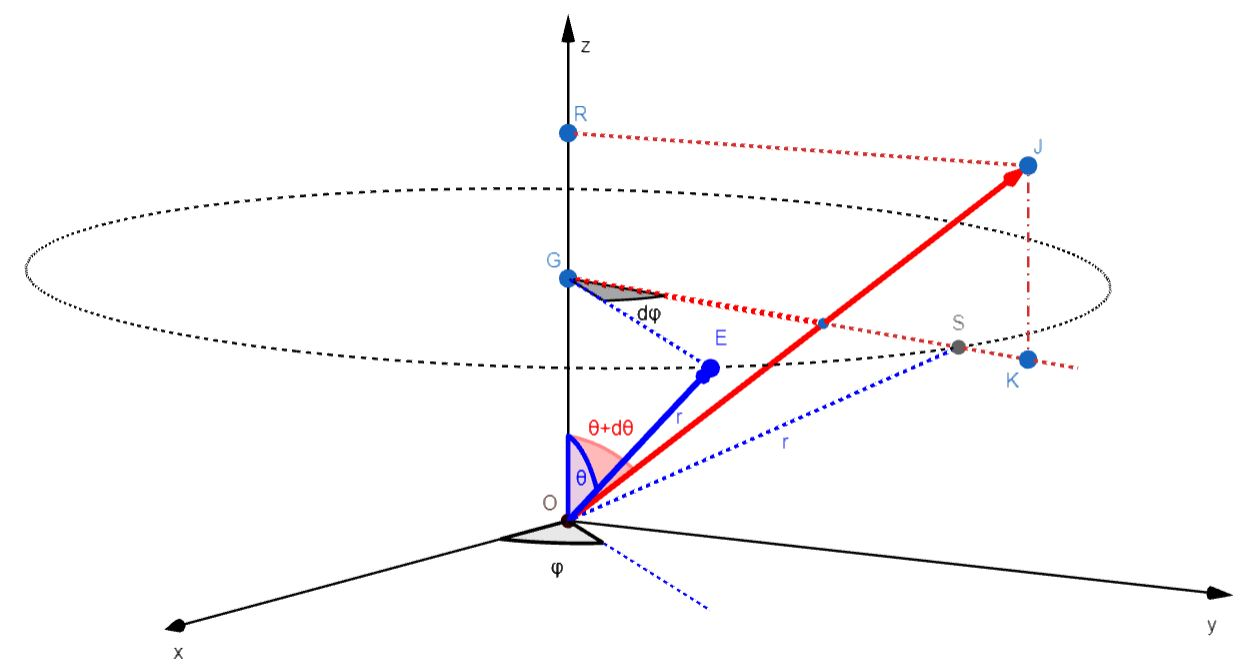
\includegraphics[scale=.6]{sphericalmetric.jpg}\\\\
Consider an infinitesimal displacement of point E to J with $(dr, d\phi , d\theta)$.
\begin{align}
\ ds^2 &= |EJ|^2
\end{align}
As we use infinitesimal displacements we can assume that $$|ES|\perp|GK|\perp|JK|\perp|ES|$$. Hence,
\begin{align}
\ ds^2 = |ES|^2+|SK|^2+|KJ|^2
\end{align}
We have the following relationships
\begin{align}
\left.
\begin{array}{c}
\ |ES| = r\sin(\phi)d\theta\\\\
\ |GE| = |GS| = r\sin(\phi)\\\\
\ |GK| = |RJ| = (r+dr)\sin(\phi+d\phi) \\
\ =(r+dr)(\cos(\phi)\sin(d\phi)+\sin(\phi)\cos(d\phi) )\\
\ = (r+dr)(\cos(\phi)d\phi+\sin(\phi))\\
\ = r\cos(\phi)d\phi+r\sin(\phi)+\sin(\phi)dr\\\\
\ |OR| =  (r+dr)\cos(\phi+d\phi)\\
\ = (r+dr)(\cos(\phi)\cos(d\phi)-\sin(\phi)\sin(d\phi))\\
\ = (r+dr)(\cos(\phi)-\sin(\phi)d\phi)\\
\ = r\cos(\phi)-r\sin(\phi)d\phi + \cos(\phi)dr\\\\
\ |OG| = r\cos(\phi)\\\\
\ |JK| = |OR|-|OG| = \cos(\phi)dr-r\sin(\phi)d\phi\\\\
\ |SK| = |GK|-|GS| = r\cos(\phi)d\phi+\sin(\phi)dr\\\\
\end{array}
\right\}
\end{align}
\begin{align}
\left.
\begin{array}{c}
\ |ES|^2 = r^2\sin^2(\phi)d\theta^2\\
\ |SK|^2 = r^2\cos^2(\phi)d\phi^2+\sin^2(\phi)dr^2 +2r\cos(\phi)\sin(\phi)drd\phi \\
\ |JK|^2 = \cos^2(\phi)dr^2+r^2\sin^2(\phi)d\phi^2 -2r\cos(\phi)\sin(\phi)drd\phi\\
\end{array}
\right\}
\end{align}
Hence,
\begin{align}
\ ds^2 &= |ES|^2+|SK|^2+|KJ|^2\\
&= \left\{ \begin{array}{c} r^2\sin^2(\phi)d\theta^2 \\ +r^2\cos^2(\phi)d\phi^2+\sin^2(\phi)dr^2 +2r\cos(\phi)\sin(\phi)drd\phi\\+r^2\sin^2(\phi)d\phi^2+\cos^2(\phi)dr^2 -2r\cos(\phi)\sin(\phi)drd\phi\\
\end{array}
\right.\\
\ &\Rightarrow ds^2= dr^2 + r^2d\phi^2 + r^2\sin^2(\phi)d\theta^2\\
\ & \Rightarrow (a_{mn}) = \begin{pmatrix}
 1& 0 & 0\\
0 & r^2 & 0 \\
0 & 0 & r^2\sin^2(\phi) \\
\end{pmatrix}
\end{align}
$$\medblackdiamond$$
\newpage


\section{p27-exercise}

\begin{tcolorbox}
Starting from 3.103, show that $$a_{mn} = \pdv{y^1}{x^m}\pdv{y^1}{x^n}+\pdv{y^2}{x^m}\pdv{y^2}{x^n}+\pdv{y^3}{x^m}\pdv{y^3}{x^n}$$ and calculate the quantities for a sphere, taking as curvilinear coordinates on he sphere $$x^1 = y^1 , x^2 = y^2$$
\end{tcolorbox}
We have
\begin{align}
\text{(2.103)}\quad &\Rightarrow y^1 = x^1 , y^2 = x^2, y^3 = f^3(x^1,x^2)\\
\text{surface = sphere}\quad &\Rightarrow y^3 = \pm \sqrt{R^2 -(x^1)^2-(x^2)^2}\\
\ ds^2 &= (dx^1)^2+(dx^2)^2+(dx^3)^2\\
\ \text{(1) and (2)}\quad& \Rightarrow \left\{ \begin{array}{c} 
\ dy^1 = dx^1\\\\
\ dy^2 = dx^2\\\\
\ dy^3 = \pm \frac{1}{2} \frac{-2x^1dx^1 - 2x^2dx^2}{\sqrt{R^2 -(x^1)^2-(x^2)^2}}\\\\
\end{array}
\right.\\
\Rightarrow ds^2 & = (dx^1)^2 +  (dx^2)^2 + \frac{(x^1)^2(dx^1)^2 + (x^2)^2(dx^2)^2  + 2 x^1x^2dx^1dx^2}{R^2 -(x^1)^2-(x^2)^2}
\end{align}
\begin{align}
\Leftrightarrow ds^2 & = \frac{(R^2 - (x^2)^2) (dx^1)^2 + (R^2 -(x^1)^2) (dx^2)^2  + 2 x^1x^2dx^1dx^2}{R^2 -(x^1)^2-(x^2)^2}
\end{align}\\
\begin{align}
\Rightarrow (a_{mn}) &= \frac{1}{R^2 -(x^1)^2-(x^2)^2}\begin{pmatrix}
 R^2 - (x^2)^2&x^1x^2 \\
x^1x^2 & R^2 - (x^1)^2 \\
\end{pmatrix}
\end{align}
$$\medblackdiamond$$
\newpage


\section{p30-clarification 2.202}

\begin{tcolorbox}
           $$\quad\quad a_{mr}\Delta^{ms} = a_{rm}\Delta^{sm} = \delta^s_r a$$
\end{tcolorbox}
Case 1: $r =s$\\
We have, $a_{Rm}\Delta^{Rm}$ (no summation on R) is the definition of the determinant of A developed along the row R: OK.\\\\
Case 2: $r \neq s$\\
Consider
\begin{align}
\ A &= \begin{pmatrix}
 a_{11} & a_{12}&\dots&a_{1N} \\
a_{21} & a_{22}&\dots&a_{2N} \\
\vdots & \vdots &\vdots & \vdots \\
a_{N1} & a_{N2}&\dots&a_{NN} \\
\end{pmatrix}
\end{align}
and consider the matrix $A^,$
\begin{align}
\ A^, &= \begin{pmatrix}
 a_{11} & a_{12}&\dots&a_{1N} \\
 \vdots & \vdots &\vdots & \vdots \\
a_{R1} & a_{R2}&\dots&a_{RN} \\
\vdots & \vdots &\vdots & \vdots \\
a_{R1} & a_{R2}&\dots&a_{RN} \\
\vdots & \vdots &\vdots & \vdots \\
a_{N1} & a_{N2}&\dots&a_{NN} \\
\end{pmatrix}
\begin{array}{c}
\ \vdots\\
\ \vdots\\
\leftarrow S^{th}\text{ row}\\
\vdots\\
\leftarrow R^{th}\text{ row}\\
\ \vdots\\
\ \vdots\\
\end{array}
\end{align}
This matrix corresponds to the way $a_{Rm}\Delta^{Sm}$ is computed. Indeed with the factor $a_{Rm}$ is not associated it's own cofactor $\Delta^{Rm}$ but the cofactor of the $m^{th}$ column in row $S$. Replacing the $S^{th}$ row with the row $R$ and calculating it's determinant is the same as calculating $a_{Rm}\Delta^{Sm}$\\
But, $|A^,| = 0$ as we have two identical rows. So, $a_{Rm}\Delta^{Sm} = 0$\\\\
Conclusion : The same reasoning can be applied when expanding the determinant along the columns instead of the rows we have indeed $\quad\quad a_{mr}\Delta^{ms} = a_{rm}\Delta^{sm} = \delta^s_r a$.
$$\medblackdiamond$$
\newpage


\section{p31-exercise}

\begin{tcolorbox}
Show that if $a{mn} = 0$ for $m\neq n$, then $$a^{11} = \frac{1}{a_{11}}, a^{22} = \frac{1}{a_{22}}, \dots, a¨{12} = 0, \dots$$
\end{tcolorbox}
We have to prove that:
\begin{align}
\ a^{ij} = \left\{\begin{array}{cc}
\frac{1}{a_{ij}} & \text{: }i=j\\
\ 0 & \text{: }i \neq j
\end{array}\right.
\end{align}
From 2.204:
\begin{align}
a_{mR}a_{mS} = \delta^S_R
\end{align}
i) Be $R \neq S$
\begin{align}
\text{(2) }\quad \Rightarrow a_{mR}a_{mS} &= 0\\
\text{but } \quad a_{mR} &=0\quad \forall m \neq R\\
\Rightarrow a_{RR}a^{RS} = 0
\end{align}
but $a_{RR} \neq 0$ ($a_{RR}$ can't be $0$ as the metric tensor would degenerate  if $a_{mn} = 0\quad \forall m \neq n$
\begin{align}
\Rightarrow a^{Rs} = 0\\\\
\end{align}

i) Be $R = S$
\begin{align}
\text{(2) }\quad \Rightarrow a_{mR}a_{mR} &= 1\\
\text{but } \quad a_{mR} &=0\quad \forall m \neq R\\
\Rightarrow a_{RR}a^{RR} = 1\\
\Rightarrow a^{RR} = \frac{1}{a_{RR}}
\end{align}
$$\medblackdiamond$$
\newpage

\section{p31-exercise}

\begin{tcolorbox}
Find the components of $a^{mn}$ for spherical polar coordinates in Eulidean 3-space.
\end{tcolorbox}
We have (see exercise page 27):
\begin{align}
\ (a_{mn}) = \begin{pmatrix}
 1& 0 & 0\\
0 & r^2 & 0 \\
0 & 0 & r^2\sin^2(\phi) \\
\end{pmatrix}
\end{align}
As $a_{mn} = 0 \quad \forall m \neq n$ we deduce (see previous exercise p31)
\begin{align}
\ (a^{mn}) = \begin{pmatrix}
 1& 0 & 0\\
0 & \frac{1}{r^2} & 0 \\
0 & 0 & \frac{1}{r^2\sin^2(\phi)}\\
\end{pmatrix}
\end{align}
$$\medblackdiamond$$
\newpage

\section{p32-exercise}

\begin{tcolorbox}
Find the mixed metric tensor  $a^{.n}_m$ obtained from $a_{mn}$ by raising the second subscript
\end{tcolorbox}
We have :
\begin{align}
\ a_{i}^{.j} &=  a_{in}a^{nj}\\
\ &=  a_{in}a^{jn}\quad a^{jn} \text{  is symmetric}\\
\ &= \delta^j_i \quad \text{ (see 2.205 pg. 30)}\\
\ &\Rightarrow a_{i}^{.j} = \delta^j_i 
\end{align}
$$\medblackdiamond$$
\newpage

\section{p33-clarification 2.214}
\begin{tcolorbox}
          $$ \pdv{a}{a_{mn}} = a a^{mn}$$
\end{tcolorbox}
Put $a_{MN}\equiv a_{mn}$. By definition, we have
\begin{align}
\  a\equiv |a_{mn}|  &= a_{Mk}\Delta^{Mk}\quad\text{(develop determinant along row M)}\\
\ &\Rightarrow \pdv{a}{a_{mn}} = \pdv{a_{Mk}}{a_{mn}}\Delta^{Mk} + a_{Mk}\pdv{\Delta^{Mk}}{a_{mn}}\\
\text{but}\quad &\pdv{a_{Mk}}{a_{mn}} = \left\{\begin{array}{c}
\ 1\quad\text{if} \quad k = N\\
\ 0\quad\text{if} \quad k \neq N\\
\end{array}\right.\\
\text{and}\quad &\pdv{\Delta^{Mk}}{a_{mn}} = 0 \quad \forall k \text{ as } \Delta^{Mk} \text{does not contain the row with } a_{mn} \text{ as element.}\\
\ & \text{(3) and (4)}\quad  \Rightarrow \pdv{a}{a_{mn}} = \Delta^{MN}\\ 
\ &  a^{mn} = \frac{\Delta^{mn}}{a}\quad\text{by definition (see 2.203 page 30)}\\
\ & \Rightarrow \pdv{a}{a_{mn}} = aa^{mn}
\end{align} 
$$\medblackdiamond$$
\newpage


\section{p32-exercise}

\begin{tcolorbox}
Prove that $a_{mn}a^{mn} = N$.
\end{tcolorbox}
From 2.204, we have
\begin{align}
\ a_{mr}a^{ms} &= \delta^s_r\\
\text{Consider} \quad a_{mR}a^{mR} &= 1\\
\text{We can repeat (2) for R = 1,2,...,N} \quad \Rightarrow a_{mr}a^{mr} &= N\\
\end{align}
$$\medblackdiamond$$
\newpage

\section{p37-exercise}

\begin{tcolorbox}
Show that the small angle between unit vectors $X^r$ and $X^r + dX^r$ (these increments being infenitesimal) is given by $$ \theta^2 = a_{mn}X^mX^n$$
\end{tcolorbox}
\begin{figure}[htp] 
    \centering
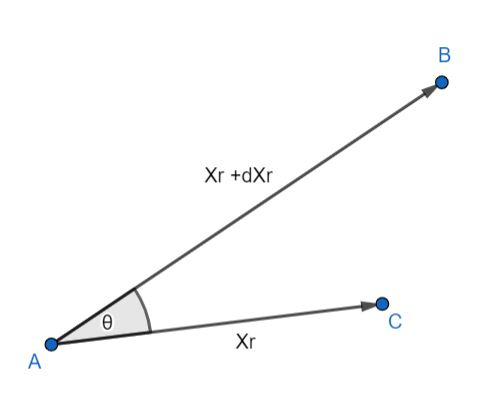
\includegraphics[scale=.5]{Exp37_1.jpg}
\end{figure}
By definition (2.302 page 33)
\begin{align} 
\ |BC|^2 =\epsilon a_{mn}dX^mdX^n\\
\end{align}
We can drop $\epsilon = 1$ as the considered space is positive definite.\\
As $\theta$ is infinitesimal, we can state
\begin{align}
\ |BC| &\approx |AC|\theta\\
\text{ and } \quad |AC| &= X^r = 1\quad  \text{(as } X^r \text{ is a unit vector)}\\
\Rightarrow \theta^2 &= a_{mn}dX^mdX^n
\end{align}
$$\medblackdiamond$$
\newpage

\section{p36-clarification 2.314}

\begin{tcolorbox}
Going from 2.313 to 2.314 yields because both $X^m$ and $Y^m$ are unit vectors and by definition of the magnitude (see 2.301) both  $a_{mn}X^mX^n$ and $a_{mn}Y^mY^n$ are 1 (also due to the fact that only a positive definite metric tensor is considered, $\epsilon = 1$).
\end{tcolorbox}
$$\medblackdiamond$$
\newpage

\section{p37-clarification 2.409}

\begin{tcolorbox}
We clarify the integration by parts in the derivation of the general  geodesic equation.
\end{tcolorbox}
We have 
\begin{align}
\int d(A.B) &= \int AdB + \int BdA\\
\Rightarrow  \int AdB &= \int BdA -  \int d(A.B)\
\end{align}
Now, substitute 2.407 in 2.406, we get
\begin{align}
\dv{L}{v} &= \int \pdv{(\epsilon w)^{\frac{1}{2}}}{x^r} \pdv{x^r}{v} du +  \int \pdv{(\epsilon w)^{\frac{1}{2}}}{p^r} \pdv{p^r}{v} du\\
\ &= \int \pdv{(\epsilon w)^{\frac{1}{2}}}{x^r} \pdv{x^r}{v} du +  \int \pdv{(\epsilon w)^{\frac{1}{2}}}{p^r} \pdv{\pdv{x^r}{v}}{u} du\\
&= \int \pdv{(\epsilon w)^{\frac{1}{2}}}{x^r} \pdv{x^r}{v} du +  \int \pdv{(\epsilon w)^{\frac{1}{2}}}{p^r} d(\pdv{x^r}{v})
\end{align}
To integrate by parts the second term in (5) we put in (2)
$$A= \pdv{(\epsilon w)^{\frac{1}{2}}}{p^r} \quad \text{and } B = \pdv{x^r}{v}$$
\begin{align}
\int \pdv{(\epsilon w)^{\frac{1}{2}}}{p^r} d(\pdv{x^r}{v}) &= \int AdB \\
\ & = \int BdA -  \int d(A.B)\\
\ &= \pdv{(\epsilon w)^{\frac{1}{2}}}{p^r}\left.\pdv{x^r}{v}\right|_{u_0}^{u_1} - \int \pdv{x^r}{v}d(\pdv{(\epsilon w)^{\frac{1}{2}}}{p^r} )\\
\ &= \pdv{(\epsilon w)^{\frac{1}{2}}}{p^r}\left.\pdv{x^r}{v}\right|_{u_0}^{u_1} - \int \pdv{x^r}{v}\pdv{\pdv{(\epsilon w)^{\frac{1}{2}}}{p^r} )}{u}du
\end{align}
Replacing (9) in (5) gives the formulea 2.409.
$$\medblackdiamond$$
\newpage